\documentclass[tikz,border=10pt]{standalone}
\usepackage{amsmath}
\usepackage{tikz}
\usetikzlibrary{arrows.meta, positioning, calc, shapes.geometric}

\begin{document}
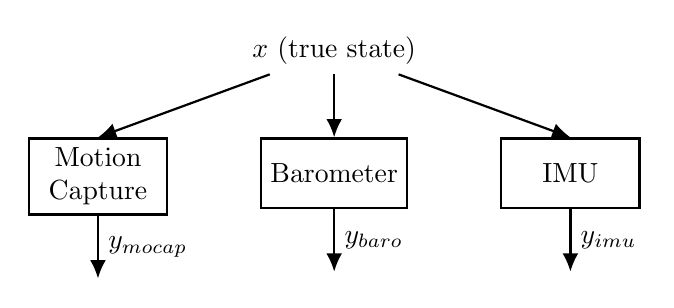
\begin{tikzpicture}[
  block/.style = {draw, thick, minimum height=2.5em, minimum width=5em, align=center},
  arrow/.style = {thick, -{Latex[width=2mm]}},
  node distance=1.5cm and 1.5cm
]

  % Input from plant
  \node (plant_out) at (0, 1.5) {$x$ (true state)};

  % Three sensor blocks
  \node[block, below=0.8cm of plant_out, xshift=-3cm] (mocap) {Motion\\Capture};
  \node[block, below=0.8cm of plant_out] (baro) {Barometer};
  \node[block, below=0.8cm of plant_out, xshift=3cm] (imu) {IMU};

  % Arrows from plant to sensors
  \draw[arrow] (plant_out) -- (mocap.north);
  \draw[arrow] (plant_out) -- (baro.north);
  \draw[arrow] (plant_out) -- (imu.north);

  % Sensor outputs
  \draw[arrow] (mocap.south) -- ++(0,-0.8) node[midway, right] {$y_{mocap}$};
  \draw[arrow] (baro.south) -- ++(0,-0.8) node[midway, right] {$y_{baro}$};
  \draw[arrow] (imu.south) -- ++(0,-0.8) node[midway, right] {$y_{imu}$};

\end{tikzpicture}
\end{document}
